\documentclass[12pt]{article}

\usepackage[utf8]{inputenc}
\usepackage[spanish]{babel}
\usepackage[vmargin=2.5cm,hmargin=2.5cm]{geometry}
\usepackage{enumerate}
\usepackage{algpseudocode}
\usepackage{graphics,graphicx,float} %para incluir imágenes y colocarlas
\usepackage{minted}
\usepackage[hidelinks]{hyperref}

\title{\vspace{4cm}
Práctica 3: Planificación\\
\vspace{1cm}
Relación de Ejercicios Entrega1:\\
Dominios y problemas de planificación
clásica en PDDL.}

\author{ Elena María Gómez Ríos }


\begin{document}


\maketitle
\newpage
% Índice
\tableofcontents
\newpage

\section{Resumen}
El objetivo de esta práctica es experimentar con el lenguaje PDDL y con el planificador Metric-FF. Se van a realizar una serie de ejercicios inspirados en ``Los extraños mundos de Belkan'', centrándonos solo en comportamientos deliberativos, en concreto comportamientos definidos mediante un dominio de planificación y especificados como planes de acciones que tiene que llevar a cabo un jugador para poder cumplir misiones en el juego.

Hay cinco personajes (Princesa, Príncipe, Bruja, Profesor y Leonardo di Caprio) y varios objetos (óscars, manzanas, rosas, algoritmos y oro).

\section{Ejercicio 1} \textbf{Definir un dominio y problema de planificación considerando que el jugador podrá estar orientado al norte, sur, este u oeste y desplazarse de una zona a otra siempre que esté correctamente orientado. Por ejemplo, podrá desplazarse a una zona al norte de su zona actual, si está orientado al norte. Realizar las siguientes tareas:}\\

Para este ejercicio he creado los archivos ``Ej1dominio.pddl'', ``Ej1problema1.pddl'' y ``Ej1problema2.pddl''.\\

\textbf{a) Representar en el dominio los objetos del mundo (jugador, personajes, tipos de objetos y las zonas del mundo).}\\

Para representar en el dominio los objetos del mundo incluimos las siguientes líneas en nuestro código:

\begin{minted}{console}
    (:types
    jugador
    orientacion
    personaje
    objeto
    zona
  )
\end{minted}

Los distintos tipos de orientación, personajes, objetos y zonas se declaran en el problema:
\begin{itemize}
	\item \textbf{orientación:} norte, sur, este y oeste
	\item \textbf{personaje:} Princesa, Príncipe, Bruja, Profesor y Leonardo di Caprio
	\item \textbf{objeto:} óscar, manzana, rosa, algoritmo y oro
	\item \textbf{zona:} un total de 25 zonas
\end{itemize}
También hará falta un jugador que es el personaje principal que debe resolver las misiones.\\

\textbf{b) Representar predicados que permitan describir los estados del mundo,
mediante la especificación de aspectos como la relación de conexión entre
zonas (representando no solo la relación de conexión, sino también que una
zona está al norte/sur/este/oeste de otra), la orientación del jugador, las
posiciones de los objetos y cualquier otra relación o propiedad que sea
necesaria para la correcta definición de las acciones que puede realizar el
jugador.}\\

Definimos un conjunto de predicados que agrupan los posibles estados en los que se encuentran los objetos:
\begin{itemize}
	\item \textbf{(nextZoneInOrientation ?z1 - zona ?o - orientacion ?z2 - zona):} este predicado indica la conexión entre dos zonas, además de la relación de orientación entre la primera zona y la segunda.
	\item \textbf{(atJugador ?j - jugador ?o - orientacion):} sirve para indicar la orientación del jugador.
	\item \textbf{(posObjeto ?o - objeto ?z - zona ):} permite indicar la posición de un objeto.
	\item \textbf{(posJugador ?j - jugador ?z - zona ):} predicado para indicar la posición del jugador.
	\item \textbf{(posPersonaje ?p - personaje ?z - zona):} predicado para indicar la posición de un personaje.
	\item \textbf{(manoVacia ?j - jugador):} indica si el jugador tiene la mano vacía.
	\item \textbf{(manoLlena ?j - jugador ?o - objeto):} indica que el jugador tiene un objeto
	\item \textbf{(entregado ?p - personaje):} indica que un personaje ya ha recibido un objeto.
	
     
\end{itemize}

\textbf{c) Representar las siguientes acciones del jugador:
i. girar a la izquierda, girar a la derecha, ir (de una zona a otra
correctamente orientado), coger (un objeto), dejar (un objeto) y
entregar (un objeto a un personaje).}

\begin{itemize}
 \item \textbf{GirarIzquierda y GirarDerecha:} para girar a la izquierda o derecha hay que tener en cuenta la orientación del jugador de la que partimos para poder dar la nueva orientación correctamente. 
 \item \textbf{Ir:} para movernos de una zona a otra es necesario conocer la orientación del jugador, la zona en la que se encuentra, la siguiente zona y si dichas zonas están conectadas por esa orientación.
 \item \textbf{Coger:} para coger un objeto es necesario que el objeto y el jugador se encuentren en la misma zona. Para que esto sea posible el jugador deberá tener las manos vacías y pasará por tanto a tener las manos llenas con dicho objeto.
 \item \textbf{Dejar:} el jugador suelta el objeto en la misma zona en la que se encuentra pasando a tener las manos vacías.
 \item \textbf{Entregar:} el jugador entrega un objeto a un personaje, para ello es necesario que el jugador se encuentre en la misma zona que el personaje y dicho personaje no haya recibido aún ningún objeto. El jugador pasa a tener las manos vacías.
\end{itemize}

\textbf{d) Plantear un problema de planificación con un estado inicial con 25 zonas
conectadas arbitrariamente en el que aparezcan situados los 5 personajes en
distintas zonas y al menos 5 objetos. El objetivo de este problema consistirá en
conseguir que todos los personajes tengan al menos un objeto. Comprobar
con Metric-FF que se obtiene un plan para conseguir esta misión.}\\

En el problema definimos los distintos objetos que son necesarios para la realización del ejercicio de la siguiente forma:

\begin{minted}{console}
      ZONE_00_00 ZONE_00_01 ZONE_00_02 ZONE_00_03 ZONE_00_04 - zona
      ZONE_01_00 ZONE_01_01 ZONE_01_02 ZONE_01_03 ZONE_01_04 - zona
      ZONE_02_00 ZONE_02_01 ZONE_02_02 ZONE_02_03 ZONE_02_04 - zona
      ZONE_03_00 ZONE_03_01 ZONE_03_02 ZONE_03_03 ZONE_03_04 - zona
      ZONE_04_00 ZONE_04_01 ZONE_04_02 ZONE_04_03 ZONE_04_04 - zona
      norte sur este oeste - orientacion
      oscar manzana rosa algoritmo oro - objeto
      Princesa Principe Bruja Profesor LeonardoDiCaprio - personaje
      jugador1 - jugador
\end{minted}

También inicializamos los objetos tal y como se muestra en la siguiente imagen:

\begin{figure}[H] 
	\centering
	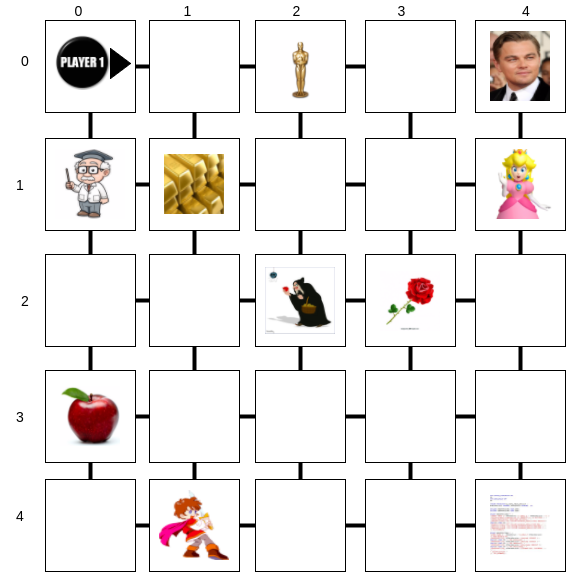
\includegraphics[width=10cm]{Ej1.png}
	\caption{Mapa problema 1}
\end{figure}

El objetivo del problema es conseguir que todos los personajes tengan un objeto, para ello hemos conseguido la siguiente solución:

\begin{minted}{console}
ff: found legal plan as follows

step    0: IR JUGADOR1 ESTE ZONE_00_00 ZONE_00_01
        1: IR JUGADOR1 ESTE ZONE_00_01 ZONE_00_02
        2: COGER JUGADOR1 ZONE_00_02 OSCAR
        3: IR JUGADOR1 ESTE ZONE_00_02 ZONE_00_03
        4: IR JUGADOR1 ESTE ZONE_00_03 ZONE_00_04
        5: GIRARDERECHA JUGADOR1 ESTE
        6: ENTREGAR OSCAR LEONARDODICAPRIO ZONE_00_04 JUGADOR1
        7: IR JUGADOR1 SUR ZONE_00_04 ZONE_01_04
        8: GIRARDERECHA JUGADOR1 SUR
        9: IR JUGADOR1 OESTE ZONE_01_04 ZONE_01_03
       10: IR JUGADOR1 OESTE ZONE_01_03 ZONE_01_02
       11: IR JUGADOR1 OESTE ZONE_01_02 ZONE_01_01
       12: COGER JUGADOR1 ZONE_01_01 ORO
       13: IR JUGADOR1 OESTE ZONE_01_01 ZONE_01_00
       14: GIRARIZQUIERDA JUGADOR1 OESTE
       15: ENTREGAR ORO PROFESOR ZONE_01_00 JUGADOR1
       16: IR JUGADOR1 SUR ZONE_01_00 ZONE_02_00
       17: IR JUGADOR1 SUR ZONE_02_00 ZONE_03_00
       18: COGER JUGADOR1 ZONE_03_00 MANZANA
       19: IR JUGADOR1 SUR ZONE_03_00 ZONE_04_00
       20: GIRARIZQUIERDA JUGADOR1 SUR
       21: IR JUGADOR1 ESTE ZONE_04_00 ZONE_04_01
       22: ENTREGAR MANZANA PRINCIPE ZONE_04_01 JUGADOR1
       23: IR JUGADOR1 ESTE ZONE_04_01 ZONE_04_02
       24: IR JUGADOR1 ESTE ZONE_04_02 ZONE_04_03
       25: IR JUGADOR1 ESTE ZONE_04_03 ZONE_04_04
       26: COGER JUGADOR1 ZONE_04_04 ALGORITMO
       27: GIRARIZQUIERDA JUGADOR1 ESTE
       28: IR JUGADOR1 NORTE ZONE_04_04 ZONE_03_04
       29: IR JUGADOR1 NORTE ZONE_03_04 ZONE_02_04
       30: IR JUGADOR1 NORTE ZONE_02_04 ZONE_01_04
       31: GIRARIZQUIERDA JUGADOR1 NORTE
       32: ENTREGAR ALGORITMO PRINCESA ZONE_01_04 JUGADOR1
       33: IR JUGADOR1 OESTE ZONE_01_04 ZONE_01_03
       34: GIRARIZQUIERDA JUGADOR1 OESTE
       35: IR JUGADOR1 SUR ZONE_01_03 ZONE_02_03
       36: COGER JUGADOR1 ZONE_02_03 ROSA
       37: GIRARDERECHA JUGADOR1 SUR
       38: IR JUGADOR1 OESTE ZONE_02_03 ZONE_02_02
       39: ENTREGAR ROSA BRUJA ZONE_02_02 JUGADOR1

\end{minted}

He realizado otro problema con la siguiente inicialización: 

\begin{figure}[H] 
	\centering
	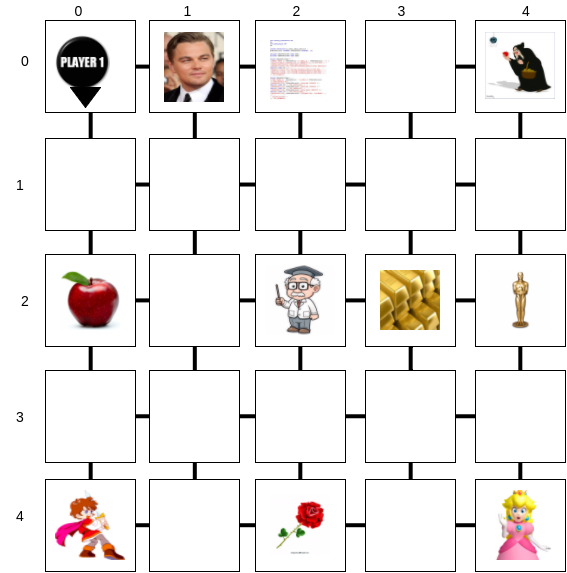
\includegraphics[width=10cm]{Ej1_2.png}
	\caption{Mapa problema 1-2}
\end{figure}

Dando la siguiente solución: 

\begin{minted}{console}
ff: found legal plan as follows

step    0: IR JUGADOR1 SUR ZONE_00_00 ZONE_01_00
        1: IR JUGADOR1 SUR ZONE_01_00 ZONE_02_00
        2: COGER JUGADOR1 ZONE_02_00 MANZANA
        3: IR JUGADOR1 SUR ZONE_02_00 ZONE_03_00
        4: IR JUGADOR1 SUR ZONE_03_00 ZONE_04_00
        5: GIRARIZQUIERDA JUGADOR1 SUR
        6: ENTREGAR MANZANA PRINCIPE ZONE_04_00 JUGADOR1
        7: IR JUGADOR1 ESTE ZONE_04_00 ZONE_04_01
        8: IR JUGADOR1 ESTE ZONE_04_01 ZONE_04_02
        9: COGER JUGADOR1 ZONE_04_02 ROSA
       10: IR JUGADOR1 ESTE ZONE_04_02 ZONE_04_03
       11: IR JUGADOR1 ESTE ZONE_04_03 ZONE_04_04
       12: GIRARIZQUIERDA JUGADOR1 ESTE
       13: ENTREGAR ROSA PRINCESA ZONE_04_04 JUGADOR1
       14: IR JUGADOR1 NORTE ZONE_04_04 ZONE_03_04
       15: IR JUGADOR1 NORTE ZONE_03_04 ZONE_02_04
       16: COGER JUGADOR1 ZONE_02_04 OSCAR
       17: GIRARIZQUIERDA JUGADOR1 NORTE
       18: IR JUGADOR1 OESTE ZONE_02_04 ZONE_02_03
       19: IR JUGADOR1 OESTE ZONE_02_03 ZONE_02_02
       20: GIRARDERECHA JUGADOR1 OESTE
       21: GIRARDERECHA JUGADOR1 NORTE
       22: ENTREGAR OSCAR PROFESOR ZONE_02_02 JUGADOR1
       23: IR JUGADOR1 ESTE ZONE_02_02 ZONE_02_03
       24: COGER JUGADOR1 ZONE_02_03 ORO
       25: IR JUGADOR1 ESTE ZONE_02_03 ZONE_02_04
       26: GIRARIZQUIERDA JUGADOR1 ESTE
       27: IR JUGADOR1 NORTE ZONE_02_04 ZONE_01_04
       28: IR JUGADOR1 NORTE ZONE_01_04 ZONE_00_04
       29: GIRARIZQUIERDA JUGADOR1 NORTE
       30: ENTREGAR ORO BRUJA ZONE_00_04 JUGADOR1
       31: IR JUGADOR1 OESTE ZONE_00_04 ZONE_00_03
       32: IR JUGADOR1 OESTE ZONE_00_03 ZONE_00_02
       33: COGER JUGADOR1 ZONE_00_02 ALGORITMO
       34: IR JUGADOR1 OESTE ZONE_00_02 ZONE_00_01
       35: ENTREGAR ALGORITMO LEONARDODICAPRIO ZONE_00_01 JUGADOR1
\end{minted}

En ambos casos podemos comprobar que nos ha dado un plan correcto entregando un objeto a cada personaje.

\section{Ejercicio 2.} \textbf{Una vez comprobado que el dominio descrito es correcto, considerar que la acción de desplazamiento entre zonas tiene un coste igual a la longitud del camino entre cada zona.}\\

Para este ejercicio he creado los archivos ``Ej2dominio.pddl'' y ``Ej2problema.pddl''.\\

\textbf{a) Modificar el dominio del anterior ejercicio para adecuarlo a esta nueva
característica.}\\

Debemos crear las siguientes funciones:

\begin{minted}{console}
  (:functions
    (camino)
    (coste ?a ?b - zona)
  )
\end{minted}

La función \texttt{(coste ?a ?b - zona)} servirá para darle a cada camino un coste específico y la función \texttt{(camino)} es la encargada de ir guardando el coste total del camino.

Además debemos cambiar la acción \texttt{Ir} para almacenar el coste del camino en la función \texttt{(camino)}, para ello he usado la función \texttt{increase} de pddl.

\begin{minted}{console}
(:action Ir
    :parameters (?j - jugador ?o - orientacion ?z1 - zona ?z2 - zona)
    :precondition 
    	(and (atJugador ?j ?o) (posJugador ?j ?z1) 
    		(nextZoneInOrientation ?z1 ?o ?z2))
    :effect 
    	(and (not (posJugador ?j ?z1)) (posJugador ?j ?z2) 
    		(increase (camino) (coste ?z1 ?z2)))
  )

\end{minted}

\textbf{b) Extender el problema definido en el anterior ejercicio, definiendo distancias
entre zonas y comprobar que el planificador obtiene un plan para estas nuevas
restricciones.}\\

En el problema he dado costes de forma aleatoria a los caminos que unen las zonas utilizando la función creada para ello \texttt{(coste ?a ?b - zona)} de la siguiente forma \texttt{(= (coste ZONE\_00\_00 ZONE\_01\_00) 10)}. También hay que tener en cuenta inicializar la función \texttt{(camino)} a 0 para poder hacer los incrementos correctamente \texttt{(= (camino) 0)}. Quedando inicializado el problema de la siguiente forma:

\begin{figure}[H] 
	\centering
	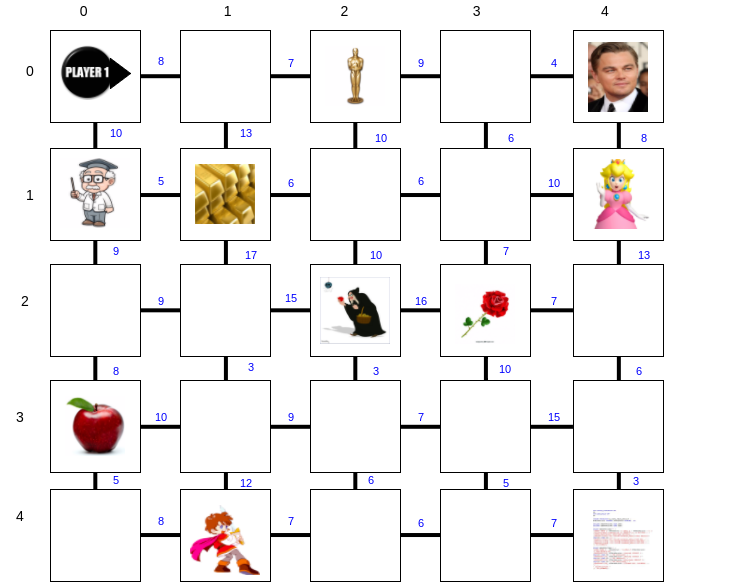
\includegraphics[width=12cm]{Ej2_1.png}
	\caption{Mapa problema ejercicio 2}
\end{figure}

\textbf{c) A partir de esta definición de problema, modificarlo de forma que el
planificador pueda encontrar el camino mínimo.}\\

Esto se consigue poniendo en la parte del problema la siguiente línea \texttt{(:metric minimize (camino))} la cual hace uso de la función metric de pddl.\\

El plan generado del problema es:
\begin{minted}{console}
acciones:   56   coste actual:  159.00    coste estimado:  159.00    tiempo:  162.47


ff: found legal plan as follows

step    0: GIRARDERECHA JUGADOR1 ESTE
        1: IR JUGADOR1 SUR ZONE_00_00 ZONE_01_00
        2: GIRARIZQUIERDA JUGADOR1 SUR
        3: IR JUGADOR1 ESTE ZONE_01_00 ZONE_01_01
        4: COGER JUGADOR1 ZONE_01_01 ORO
        5: GIRARDERECHA JUGADOR1 ESTE
        6: GIRARDERECHA JUGADOR1 SUR
        7: IR JUGADOR1 OESTE ZONE_01_01 ZONE_01_00
        8: GIRARIZQUIERDA JUGADOR1 OESTE
        9: ENTREGAR ORO PROFESOR ZONE_01_00 JUGADOR1
       10: IR JUGADOR1 SUR ZONE_01_00 ZONE_02_00
       11: IR JUGADOR1 SUR ZONE_02_00 ZONE_03_00
       12: COGER JUGADOR1 ZONE_03_00 MANZANA
       13: IR JUGADOR1 SUR ZONE_03_00 ZONE_04_00
       14: GIRARIZQUIERDA JUGADOR1 SUR
       15: IR JUGADOR1 ESTE ZONE_04_00 ZONE_04_01
       16: ENTREGAR MANZANA PRINCIPE ZONE_04_01 JUGADOR1
       17: IR JUGADOR1 ESTE ZONE_04_01 ZONE_04_02
       18: IR JUGADOR1 ESTE ZONE_04_02 ZONE_04_03
       19: IR JUGADOR1 ESTE ZONE_04_03 ZONE_04_04
       20: COGER JUGADOR1 ZONE_04_04 ALGORITMO
       21: GIRARIZQUIERDA JUGADOR1 ESTE
       22: GIRARIZQUIERDA JUGADOR1 NORTE
       23: IR JUGADOR1 OESTE ZONE_04_04 ZONE_04_03
       24: GIRARDERECHA JUGADOR1 OESTE
       25: IR JUGADOR1 NORTE ZONE_04_03 ZONE_03_03
       26: GIRARIZQUIERDA JUGADOR1 NORTE
       27: IR JUGADOR1 OESTE ZONE_03_03 ZONE_03_02
       28: GIRARDERECHA JUGADOR1 OESTE
       29: IR JUGADOR1 NORTE ZONE_03_02 ZONE_02_02
       30: GIRARIZQUIERDA JUGADOR1 NORTE
       31: GIRARIZQUIERDA JUGADOR1 OESTE
       32: ENTREGAR ALGORITMO BRUJA ZONE_02_02 JUGADOR1
       33: GIRARIZQUIERDA JUGADOR1 SUR
       34: IR JUGADOR1 ESTE ZONE_02_02 ZONE_02_03
       35: GIRARIZQUIERDA JUGADOR1 ESTE
       36: COGER JUGADOR1 ZONE_02_03 ROSA
       37: IR JUGADOR1 NORTE ZONE_02_03 ZONE_01_03
       38: GIRARDERECHA JUGADOR1 NORTE
       39: IR JUGADOR1 ESTE ZONE_01_03 ZONE_01_04
       40: GIRARIZQUIERDA JUGADOR1 ESTE
       41: ENTREGAR ROSA PRINCESA ZONE_01_04 JUGADOR1
       42: IR JUGADOR1 NORTE ZONE_01_04 ZONE_00_04
       43: GIRARIZQUIERDA JUGADOR1 NORTE
       44: IR JUGADOR1 OESTE ZONE_00_04 ZONE_00_03
       45: IR JUGADOR1 OESTE ZONE_00_03 ZONE_00_02
       46: COGER JUGADOR1 ZONE_00_02 OSCAR
       47: GIRARIZQUIERDA JUGADOR1 OESTE
       48: GIRARIZQUIERDA JUGADOR1 SUR
       49: IR JUGADOR1 ESTE ZONE_00_02 ZONE_00_03
       50: IR JUGADOR1 ESTE ZONE_00_03 ZONE_00_04
       51: DEJAR JUGADOR1 ZONE_00_04 OSCAR
       52: GIRARIZQUIERDA JUGADOR1 ESTE
       53: GIRARIZQUIERDA JUGADOR1 NORTE
       54: COGER JUGADOR1 ZONE_00_04 OSCAR
       55: ENTREGAR OSCAR LEONARDODICAPRIO ZONE_00_04 JUGADOR1
     		Coste Total: 159.00

\end{minted}

\section{Ejercicio 3} \textbf{Considerar ahora que (1) hay distintos tipos de zonas dependiendo del tipo de superficie que contengan, en concreto: Bosque, Agua, Precipicio, Arena y Piedra, y (2) hay dos nuevos tipos de objetos: Zapatilla y Bikini. Además, considerar también que el jugador, aparte de poder tener cogido un objeto, está dotado de una mochila donde puede guardar otro objeto (solo uno). Realizar lo siguiente:}\\

Para este ejercicio he creado los archivos ``Ej3dominio.pddl'' y ``Ej3problema.pddl''.\\

\textbf{a) Modificar el dominio del ejercicio anterior para que el jugador pueda desplazarse por el entorno considerando las siguientes restricciones:}\\

\textbf{i. Puede moverse a una zona de bosque sólo si tiene una zapatilla (cogida o en la mochila). (Puede definirse un predicado que permita determinar de qué tipo es un determinado objeto).}

\textbf{ii. Puede moverse a una zona de agua si tiene un bikini (cogido o en la mochila).}

\textbf{iii. No puede moverse a un precipicio.}\\

Lo primero que debo hacer es crear dos nuevos tipos \texttt{mochila} y \texttt{tipoterreno}. También se deben añadir los siguientes predicados:
\begin{itemize}
	\item \textbf{(mochilaVacia ?m - mochila):} indica si la mochila está vacía.
	\item \textbf{(mochilaLlena ?m - mochila ?o - objeto):} indica que la mochila tiene un objeto.
	\item \textbf{(isZone ?z - zona ?t - tipoterreno):} asigna un tipoterreno a una zona.
	
Actualizamos la acción de \texttt{Ir} para contemplar las nuevas características descritas arriba quedando de la siguiente forma:

\begin{minted}{console}
 (:action Ir
    :parameters 
    	(?j - jugador ?o - orientacion ?z1 - zona ?z2 - zona 
    	?t - tipoterreno ?m - mochila)
    :precondition
      (and
         (atJugador ?j ?o) (posJugador ?j ?z1) (nextZoneInOrientation ?z1 ?o ?z2) 	
         (isZone ?z2 ?t) (not (= ?t Precipicio))
            (or
               (and (= ?t Bosque) 
               	(or (manoLlena ?j zapatillas) (mochilaLlena ?m zapatillas)))
               (and (= ?t Agua) 
               	(or (manoLlena ?j bikini) (mochilaLlena ?m bikini)))
               (and (or (= ?t Piedra) (= ?t Arena)))
            )
      )
    :effect 
    	(and 
    		(not (posJugador ?j ?z1)) (posJugador ?j ?z2) 
    		(increase (camino) (coste ?z1 ?z2)))
  )
\end{minted}

Ahora en la precondición debemos tener en cuenta a que tipo de terreno vamos, y si vamos a bosque o agua debemos tener zapatillas o bikini respectivamente , ya sea en la mano o en la mochila, para poder acceder a dichas zonas.
     
     
\end{itemize}

\textbf{b) Modificar el domino para que pueda meter y sacar objetos en/de la mochila. Tener en cuenta que para meter en la mochila lo tiene que tener cogido, solo puede tener cogido un objeto a la vez y uno en la mochila.}\\

Añadimos dos nuevas acciones \texttt{Guardar} y \texttt{Sacar} para poder guardar y sacar objetos de la mochila:

\begin{minted}{console}
(:action Guardar
  :parameters (?j - jugador ?m - mochila ?o - objeto)
  :precondition (and (mochilaVacia ?m) (manoLlena ?j ?o))
  :effect 
    (and 
      (not (mochilaVacia ?m)) (mochilaLlena ?m ?o) 
      (manoVacia ?j) (not (manoLlena ?j ?o))
    )
)

(:action Sacar
  :parameters (?j - jugador ?m - mochila ?o - objeto)
  :precondition (and (manoVacia ?j) (mochilaLlena ?m ?o))
  :effect 
    (and 
      (manoLlena ?j ?o) (not (manoVacia ?j)) 
      (not (mochilaLlena ?m ?o)) (mochilaVacia ?m)
    )
)
\end{minted}

Debemos comprobar antes de guardar un objeto que la mochila esté vacía y que tengamos un objeto en la mano para poder guardarlo en la mochila, igualmente para sacar un objeto de la mochila debemos comprobar tener las manos vacías y que la mochila esté llena. Como tengo dos predicados para la facilidad de comprensión del código, debo comprobarlo tanto en \texttt{mochilaVacia} como en \texttt{mochilaLlena}, y de igual forma en \texttt{manoVacia} como en \texttt{manoLlena}.\\


\textbf{c) Extender el problema del anterior ejercicio para poder representar un escenario que contenga zonas de los distintos tipos descritos y también objetos de tipo zapatilla y bikini para que el jugador pueda moverse por todas las zonas. Representar al menos que hay una zapatilla en una zona de agua, o un bikini en una zona de bosque.}\\

Para el problema he añadido los terrenos y los nuevos objetos bikini y zapatillas tal y como se muestra en la siguiente imagen:


\begin{figure}[H] 
	\centering
	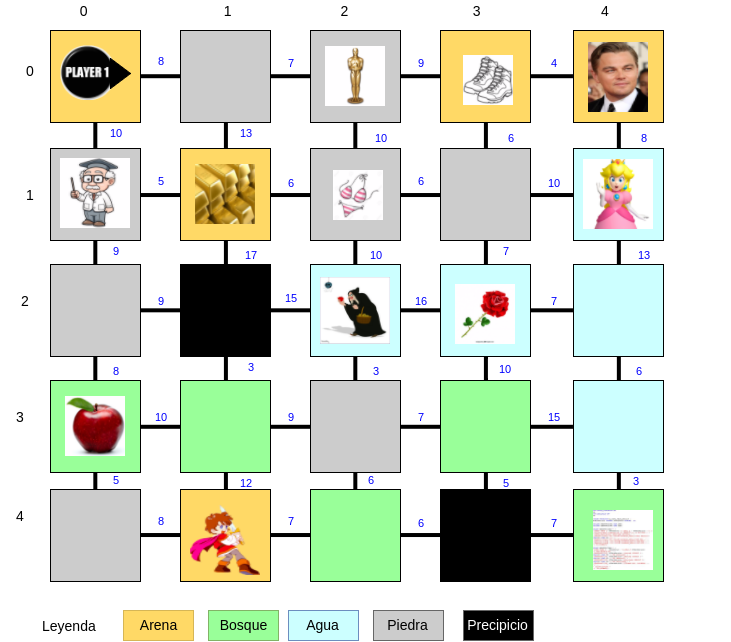
\includegraphics[width=15cm]{Ej3_1.png}
	\caption{Mapa problema ejercicio 3}
\end{figure}

El plan lo he realizado con objetivo entregar a la princesa y al príncipe, ya que si pongo como objetivo entregar a los 5 personajes tarda mucho la ejecución. De esta forma se puede ver el correcto funcionamiento ya que la princesa está en zona de agua y por lo tanto es necesario el bikini, y el príncipe está rodeado de bosque y son necesarias las zapatillas para poder entregarle un objeto. Utilizo el mismo mapa que en el ejercicio anterior.

\begin{minted}{console}
acciones:   57   coste actual:   92.00    coste estimado:   92.00    tiempo:    8.85


ff: found legal plan as follows

step    0: GIRARDERECHA JUGADOR1 ESTE
        1: IR JUGADOR1 SUR ZONE_00_00 ZONE_01_00 PIEDRA MOCHILA
        2: GIRARIZQUIERDA JUGADOR1 SUR
        3: IR JUGADOR1 ESTE ZONE_01_00 ZONE_01_01 ARENA MOCHILA
        4: COGER JUGADOR1 ZONE_01_01 ORO
        5: IR JUGADOR1 ESTE ZONE_01_01 ZONE_01_02 PIEDRA MOCHILA
        6: DEJAR JUGADOR1 ZONE_01_02 ORO
        7: COGER JUGADOR1 ZONE_01_02 BIKINI
        8: GUARDAR JUGADOR1 MOCHILA BIKINI
        9: COGER JUGADOR1 ZONE_01_02 ORO
       10: IR JUGADOR1 ESTE ZONE_01_02 ZONE_01_03 PIEDRA MOCHILA
       11: IR JUGADOR1 ESTE ZONE_01_03 ZONE_01_04 AGUA MOCHILA
       12: GIRARIZQUIERDA JUGADOR1 ESTE
       13: ENTREGAR ORO PRINCESA ZONE_01_04 JUGADOR1
       14: IR JUGADOR1 NORTE ZONE_01_04 ZONE_00_04 ARENA MOCHILA
       15: GIRARIZQUIERDA JUGADOR1 NORTE
       16: IR JUGADOR1 OESTE ZONE_00_04 ZONE_00_03 ARENA MOCHILA
       17: GIRARDERECHA JUGADOR1 OESTE
       18: SACAR JUGADOR1 MOCHILA BIKINI
       19: DEJAR JUGADOR1 ZONE_00_03 BIKINI
       20: COGER JUGADOR1 ZONE_00_03 ZAPATILLAS
       21: GUARDAR JUGADOR1 MOCHILA ZAPATILLAS
       22: COGER JUGADOR1 ZONE_00_03 BIKINI
       23: GIRARIZQUIERDA JUGADOR1 NORTE
       24: GIRARIZQUIERDA JUGADOR1 OESTE
       25: IR JUGADOR1 SUR ZONE_00_03 ZONE_01_03 PIEDRA MOCHILA
       26: IR JUGADOR1 SUR ZONE_01_03 ZONE_02_03 AGUA MOCHILA
       27: GIRARDERECHA JUGADOR1 SUR
       28: DEJAR JUGADOR1 ZONE_02_03 BIKINI
       29: COGER JUGADOR1 ZONE_02_03 ROSA
       30: GIRARIZQUIERDA JUGADOR1 OESTE
       31: IR JUGADOR1 SUR ZONE_02_03 ZONE_03_03 BOSQUE MOCHILA
       32: GIRARDERECHA JUGADOR1 SUR
       33: GIRARDERECHA JUGADOR1 OESTE
       34: DEJAR JUGADOR1 ZONE_03_03 ROSA
       35: SACAR JUGADOR1 MOCHILA ZAPATILLAS
       36: DEJAR JUGADOR1 ZONE_03_03 ZAPATILLAS
       37: COGER JUGADOR1 ZONE_03_03 ROSA
       38: GUARDAR JUGADOR1 MOCHILA ROSA
       39: COGER JUGADOR1 ZONE_03_03 ZAPATILLAS
       40: GIRARIZQUIERDA JUGADOR1 NORTE
       41: IR JUGADOR1 OESTE ZONE_03_03 ZONE_03_02 PIEDRA MOCHILA
       42: GIRARIZQUIERDA JUGADOR1 OESTE
       43: IR JUGADOR1 SUR ZONE_03_02 ZONE_04_02 BOSQUE MOCHILA
       44: DEJAR JUGADOR1 ZONE_04_02 ZAPATILLAS
       45: SACAR JUGADOR1 MOCHILA ROSA
       46: DEJAR JUGADOR1 ZONE_04_02 ROSA
       47: COGER JUGADOR1 ZONE_04_02 ZAPATILLAS
       48: GUARDAR JUGADOR1 MOCHILA ZAPATILLAS
       49: COGER JUGADOR1 ZONE_04_02 ROSA
       50: GIRARDERECHA JUGADOR1 SUR
       51: IR JUGADOR1 OESTE ZONE_04_02 ZONE_04_01 ARENA MOCHILA
       52: DEJAR JUGADOR1 ZONE_04_01 ROSA
       53: SACAR JUGADOR1 MOCHILA ZAPATILLAS
       54: DEJAR JUGADOR1 ZONE_04_01 ZAPATILLAS
       55: COGER JUGADOR1 ZONE_04_01 ROSA
       56: ENTREGAR ROSA PRINCIPE ZONE_04_01 JUGADOR1
     		Coste Total: 92.00

\end{minted}

Se puede apreciar como solo va a una zona de agua cuando tiene el bikini o a una zona de bosque cuando posee unas zapatillas. Igualmente se puede observar como guarda y saca objetos de la mochila.

\section{Ejercicio 4} \textbf{Considerar ahora que cuando el jugador entrega objetos a un personaje consigue puntos, según la siguiente tabla:}

\begin{table}[H]
\centering
\begin{tabular}{c|c|c|c|c|c|}
\cline{2-6}
                                & Leonardo & Princesa & Bruja & Profesor & Príncipe \\ \hline
\multicolumn{1}{|c|}{Oscar}     & 10       & 5        & 4     & 3        & 1        \\ \hline
\multicolumn{1}{|c|}{Rosa}      & 1        & 10       & 5     & 4        & 3        \\ \hline
\multicolumn{1}{|c|}{Manzana}   & 3        & 1        & 10    & 5        & 4        \\ \hline
\multicolumn{1}{|c|}{Algoritmo} & 4        & 3        & 1     & 10       & 5        \\ \hline
\multicolumn{1}{|c|}{Oro}       & 5        & 4        & 3     & 1        & 10       \\ \hline
\end{tabular}
\end{table}

\textbf{a) Modificar el dominio para poder registrar los puntos acumulados por el agente, mediante una función, cada vez que entrega un objeto a un personaje (una función PDDL puede tener dos argumentos).}\\

Para guardar los puntos acumulados creamos una nueva función \texttt{(puntos)} en el dominio, y para guardar los puntos correspondientes a la entrega de cada objeto a un personaje creamos la función \texttt{(puntosPersonaje ?p - personaje ?o - objeto)}.\\

\textbf{b) Extender el problema del anterior ejercicio para que, por un lado, se pueda representar la tabla anterior y, además, partiendo de 0 puntos el jugador pueda alcanzar al menos una cantidad arbitraria de puntos (indicándolo en el objetivo), sin especificar a qué personajes hay que entregar objetos. Por ejemplo, plantear un problema en el que con solo objetos de tipo oscar y manzana el jugador pueda alcanzar 50 puntos (asumiendo que solo están los 5 personajes).}\\

Para representar la tabla anterior se ha añadido en el problema todos los puntos correspondientes a la tabla de la siguiente forma: \texttt{(= (puntosPersonaje LeonardoDiCaprio oscar) 10)}. En la acción \texttt{Entregar} el incremento de la función \texttt{puntos} dependiendo del objeto y a que personaje se lo entregues:
\texttt{(increase (puntos) (puntosPersonaje ?p ?o))}

En el problema añadimos que partimos de 0 puntos al iniciar \texttt{(= (puntos) 0)} y en el goal ponemos \texttt{(AND (= (puntos) 50))} para cambiar el objetivo del problema.\\

El siguiente plan es de obtener 18 puntos, pudiendo entregar varios objetos al mismo personaje, utilizando el mismo mapa que en el ejercicio 3.
\begin{minted}{console}
ff: found legal plan as follows

step    0: IR JUGADOR1 ESTE ZONE_00_00 ZONE_00_01 PIEDRA MOCHILA
        1: GIRARDERECHA JUGADOR1 ESTE
        2: IR JUGADOR1 SUR ZONE_00_01 ZONE_01_01 ARENA MOCHILA
        3: GIRARIZQUIERDA JUGADOR1 SUR
        4: COGER JUGADOR1 ZONE_01_01 ORO
        5: IR JUGADOR1 ESTE ZONE_01_01 ZONE_01_02 PIEDRA MOCHILA
        6: DEJAR JUGADOR1 ZONE_01_02 ORO
        7: GIRARDERECHA JUGADOR1 ESTE
        8: COGER JUGADOR1 ZONE_01_02 BIKINI
        9: GUARDAR JUGADOR1 MOCHILA BIKINI
       10: COGER JUGADOR1 ZONE_01_02 ORO
       11: IR JUGADOR1 SUR ZONE_01_02 ZONE_02_02 AGUA MOCHILA
       12: GIRARIZQUIERDA JUGADOR1 SUR
       13: DEJAR JUGADOR1 ZONE_02_02 ORO
       14: GIRARIZQUIERDA JUGADOR1 ESTE
       15: IR JUGADOR1 NORTE ZONE_02_02 ZONE_01_02 PIEDRA MOCHILA
       16: IR JUGADOR1 NORTE ZONE_01_02 ZONE_00_02 PIEDRA MOCHILA
       17: COGER JUGADOR1 ZONE_00_02 OSCAR
       18: GIRARDERECHA JUGADOR1 NORTE
       19: IR JUGADOR1 ESTE ZONE_00_02 ZONE_00_03 ARENA MOCHILA
       20: IR JUGADOR1 ESTE ZONE_00_03 ZONE_00_04 ARENA MOCHILA
       21: GIRARDERECHA JUGADOR1 ESTE
       22: ENTREGAR OSCAR LEONARDODICAPRIO ZONE_00_04 JUGADOR1
       23: IR JUGADOR1 SUR ZONE_00_04 ZONE_01_04 AGUA MOCHILA
       24: IR JUGADOR1 SUR ZONE_01_04 ZONE_02_04 AGUA MOCHILA
       25: GIRARDERECHA JUGADOR1 SUR
       26: IR JUGADOR1 OESTE ZONE_02_04 ZONE_02_03 AGUA MOCHILA
       27: COGER JUGADOR1 ZONE_02_03 ROSA
       28: IR JUGADOR1 OESTE ZONE_02_03 ZONE_02_02 AGUA MOCHILA
       29: ENTREGAR ROSA BRUJA ZONE_02_02 JUGADOR1
       30: COGER JUGADOR1 ZONE_02_02 ORO
       31: ENTREGAR ORO BRUJA ZONE_02_02 JUGADOR1

\end{minted}

\section{Ejercicio 5}\textbf{Considerar ahora que el jugador tiene una mochila con una capacidad n $>$ 1, (configurable en el estado inicial).}\\

\textbf{a) Modificar el dominio y, en concreto, las acciones de desplazamiento, carga y
descarga de la mochila de acuerdo a este nuevo elemento del jugador.}\\

Creamos una nueva función, \texttt{(capacidad ?m - mochila)}, para poder asignarle una capacidad a la mochila, también creamos la función \texttt{(usoMochila)} la cual nos indica cuantos objetos hay en la mochila. El predicado mochilaVacia lo elimino, ya que si el usoMochila es 0 la mochila esta vacía.\\

Las acciones \texttt{Guardar} y \texttt{Sacar} quedarían de la siguiente forma:

\begin{minted}{console}
;Guardar objeto en la mochila
  (:action Guardar
     :parameters (?j - jugador ?m - mochila ?o - objeto)
     :precondition (and (manoLlena ?j ?o) (< (usoMochila) (capacidad ?m)) )
     :effect
      (and
         (mochilaLlena ?m ?o)
         (manoVacia ?j)
         (not (manoLlena ?j ?o))
         (increase (usoMochila) 1)
      )
  )


  ;Sacar objeto de la mochila
  (:action Sacar
     :parameters (?j - jugador ?m - mochila ?o - objeto)
     :precondition (and (manoVacia ?j) (mochilaLlena ?m ?o) (> (usoMochila) 0) )
     :effect
         (and
            (manoLlena ?j ?o)
            (not (manoVacia ?j))
            (decrease (usoMochila) 1)
            (not (mochilaLlena ?m ?o)))
         )
  )
\end{minted}

Para poder guardar un objeto en la mochila debemos comprobar la mochila no esta llena, \texttt{(< (usoMochila) (capacidad ?m))}, e incrementamos el uso de la mochila, \texttt{(increase (usoMochila) 1)}. Para poder sacar un objeto de la mochila debemos comprobar que la mochila no está vacía ,\texttt{(> (usoMochila) 0)}, y decrementamos el uso de la mochila.\\

He realizado varias pruebas para comprobar que la acción Ir funciona perfectamente también con una mochila de capacidad n $>$ 1, por lo tanto no es necesario modificar la versión del ejercicio anterior.\\

\textbf{b) Extender el problema del anterior ejercicio para que el planificador pueda
encontrar un plan con estas nuevas condiciones. Comprobar
experimentalmente que el plan obtenido en el ejercicio anterior es más largo
(contiene más acciones) que el obtenido en este ejercicio.}\\

Efectivamente el plan obtenido es mas corto que en el ejercicio anterior, esta es la solución que me da para un objetivo de 30 puntos con una capacidad de la mochila de 5. En el problema inicializamos (= (capacidad mochila) 5)
      (= (usoMochila) 0).

\begin{minted}{console}
ff: found legal plan as follows

step    0: IR JUGADOR1 ESTE ZONE_00_00 ZONE_00_01 PIEDRA MOCHILA
        1: IR JUGADOR1 ESTE ZONE_00_01 ZONE_00_02 PIEDRA MOCHILA
        2: COGER JUGADOR1 ZONE_00_02 OSCAR
        3: IR JUGADOR1 ESTE ZONE_00_02 ZONE_00_03 ARENA MOCHILA
        4: IR JUGADOR1 ESTE ZONE_00_03 ZONE_00_04 ARENA MOCHILA
        5: GIRARIZQUIERDA JUGADOR1 ESTE
        6: GIRARIZQUIERDA JUGADOR1 NORTE
        7: ENTREGAR OSCAR LEONARDODICAPRIO ZONE_00_04 JUGADOR1
        8: IR JUGADOR1 OESTE ZONE_00_04 ZONE_00_03 ARENA MOCHILA
        9: COGER JUGADOR1 ZONE_00_03 ZAPATILLAS
       10: IR JUGADOR1 OESTE ZONE_00_03 ZONE_00_02 PIEDRA MOCHILA
       11: GUARDAR JUGADOR1 MOCHILA ZAPATILLAS
       12: GIRARIZQUIERDA JUGADOR1 OESTE
       13: IR JUGADOR1 SUR ZONE_00_02 ZONE_01_02 PIEDRA MOCHILA
       14: COGER JUGADOR1 ZONE_01_02 BIKINI
       15: IR JUGADOR1 SUR ZONE_01_02 ZONE_02_02 AGUA MOCHILA
       16: GUARDAR JUGADOR1 MOCHILA BIKINI
       17: IR JUGADOR1 SUR ZONE_02_02 ZONE_03_02 PIEDRA MOCHILA
       18: GIRARDERECHA JUGADOR1 SUR
       19: IR JUGADOR1 OESTE ZONE_03_02 ZONE_03_01 BOSQUE MOCHILA
       20: IR JUGADOR1 OESTE ZONE_03_01 ZONE_03_00 BOSQUE MOCHILA
       21: GIRARDERECHA JUGADOR1 OESTE
       22: COGER JUGADOR1 ZONE_03_00 MANZANA
       23: GIRARDERECHA JUGADOR1 NORTE
       24: IR JUGADOR1 ESTE ZONE_03_00 ZONE_03_01 BOSQUE MOCHILA
       25: IR JUGADOR1 ESTE ZONE_03_01 ZONE_03_02 PIEDRA MOCHILA
       26: GIRARIZQUIERDA JUGADOR1 ESTE
       27: IR JUGADOR1 NORTE ZONE_03_02 ZONE_02_02 AGUA MOCHILA
       28: GIRARDERECHA JUGADOR1 NORTE
       29: ENTREGAR MANZANA BRUJA ZONE_02_02 JUGADOR1
       30: IR JUGADOR1 ESTE ZONE_02_02 ZONE_02_03 AGUA MOCHILA
       31: COGER JUGADOR1 ZONE_02_03 ROSA
       32: IR JUGADOR1 ESTE ZONE_02_03 ZONE_02_04 AGUA MOCHILA
       33: GIRARIZQUIERDA JUGADOR1 ESTE
       34: IR JUGADOR1 NORTE ZONE_02_04 ZONE_01_04 AGUA MOCHILA
       35: ENTREGAR ROSA PRINCESA ZONE_01_04 JUGADOR1

\end{minted}

El siguiente plan es de conseguir 18 puntos, en el ejercicio anterior necesitó 31 pasos para llegar al objetivo, en cambio en este con una mochila de capacidad 5 ha necesitado 26 pasos.
\begin{minted}{console}
ff: found legal plan as follows

step    0: IR JUGADOR1 ESTE ZONE_00_00 ZONE_00_01 PIEDRA MOCHILA
        1: GIRARDERECHA JUGADOR1 ESTE
        2: IR JUGADOR1 SUR ZONE_00_01 ZONE_01_01 ARENA MOCHILA
        3: GIRARIZQUIERDA JUGADOR1 SUR
        4: COGER JUGADOR1 ZONE_01_01 ORO
        5: IR JUGADOR1 ESTE ZONE_01_01 ZONE_01_02 PIEDRA MOCHILA
        6: GIRARIZQUIERDA JUGADOR1 ESTE
        7: GUARDAR JUGADOR1 MOCHILA ORO
        8: COGER JUGADOR1 ZONE_01_02 BIKINI
        9: IR JUGADOR1 NORTE ZONE_01_02 ZONE_00_02 PIEDRA MOCHILA
       10: GUARDAR JUGADOR1 MOCHILA BIKINI
       11: COGER JUGADOR1 ZONE_00_02 OSCAR
       12: GIRARDERECHA JUGADOR1 NORTE
       13: GIRARDERECHA JUGADOR1 ESTE
       14: IR JUGADOR1 SUR ZONE_00_02 ZONE_01_02 PIEDRA MOCHILA
       15: IR JUGADOR1 SUR ZONE_01_02 ZONE_02_02 AGUA MOCHILA
       16: ENTREGAR OSCAR BRUJA ZONE_02_02 JUGADOR1
       17: GIRARIZQUIERDA JUGADOR1 SUR
       18: IR JUGADOR1 ESTE ZONE_02_02 ZONE_02_03 AGUA MOCHILA
       19: COGER JUGADOR1 ZONE_02_03 ROSA
       20: IR JUGADOR1 ESTE ZONE_02_03 ZONE_02_04 AGUA MOCHILA
       21: GIRARIZQUIERDA JUGADOR1 ESTE
       22: IR JUGADOR1 NORTE ZONE_02_04 ZONE_01_04 AGUA MOCHILA
       23: GIRARIZQUIERDA JUGADOR1 NORTE
       24: ENTREGAR ROSA PRINCESA ZONE_01_04 JUGADOR1
       25: SACAR JUGADOR1 MOCHILA ORO
       26: ENTREGAR ORO PRINCESA ZONE_01_04 JUGADOR1

\end{minted}


\section{Ejercicio 6} \textbf{Con el dominio definido en el anterior ejercicio definir 3 problemas con
distintas capacidades de la mochila y con distinto número de objetos a entregar, de
forma que el planificador encuentre un plan para ellos maximizando el número de
puntos a conseguir.}\\

Para este ejercicio utilizo el mismo dominio del ejercicio 5 ``Ej5dominio.pddl'' y creo 3 nuevos archivos ``Ej6problema1.pddl'', ``Ej6problema2.pddl'' y ``Ej6problema3.pddl''.\\

El mapa que voy a utilizar para los dos primero problemas en este ejercicio es el siguiente:


\begin{figure}[H] 
	\centering
	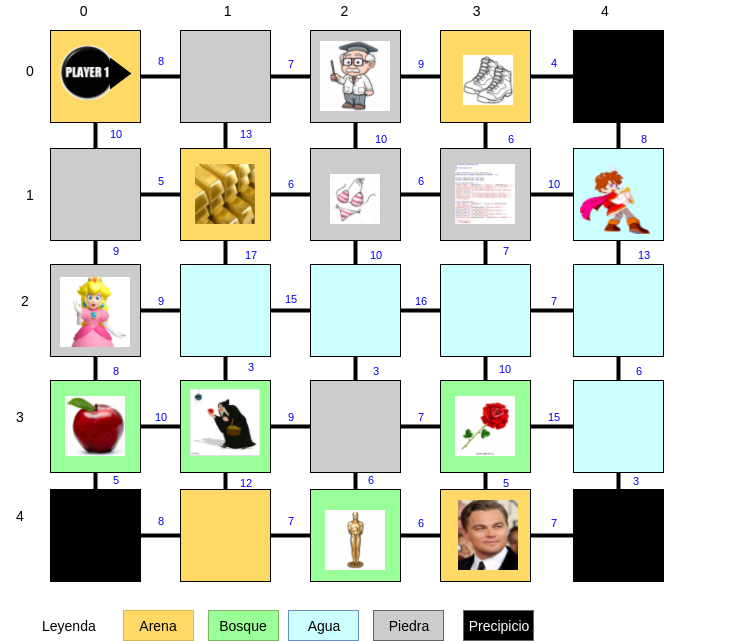
\includegraphics[width=15cm]{Ej6_1.png}
	\caption{Mapa problema ejercicio 6}
\end{figure}

En el primer problema utilizo una mochila de capacidad 2 y utilizo 2 objetos a entregar el oro y el algoritmo, el plan resultante es el siguiente:
\begin{minted}{console}
ff: found legal plan as follows

step    0: IR JUGADOR1 ESTE ZONE_00_00 ZONE_00_01 PIEDRA MOCHILA
        1: GIRARDERECHA JUGADOR1 ESTE
        2: IR JUGADOR1 SUR ZONE_00_01 ZONE_01_01 ARENA MOCHILA
        3: GIRARIZQUIERDA JUGADOR1 SUR
        4: COGER JUGADOR1 ZONE_01_01 ORO
        5: IR JUGADOR1 ESTE ZONE_01_01 ZONE_01_02 PIEDRA MOCHILA
        6: GUARDAR JUGADOR1 MOCHILA ORO
        7: COGER JUGADOR1 ZONE_01_02 BIKINI
        8: IR JUGADOR1 ESTE ZONE_01_02 ZONE_01_03 PIEDRA MOCHILA
        9: IR JUGADOR1 ESTE ZONE_01_03 ZONE_01_04 AGUA MOCHILA
       10: DEJAR JUGADOR1 ZONE_01_04 BIKINI
       11: SACAR JUGADOR1 MOCHILA ORO
       12: GIRARIZQUIERDA JUGADOR1 ESTE
       13: GIRARIZQUIERDA JUGADOR1 NORTE
       14: ENTREGAR ORO PRINCIPE ZONE_01_04 JUGADOR1
       15: IR JUGADOR1 OESTE ZONE_01_04 ZONE_01_03 PIEDRA MOCHILA
       16: COGER JUGADOR1 ZONE_01_03 ALGORITMO
       17: IR JUGADOR1 OESTE ZONE_01_03 ZONE_01_02 PIEDRA MOCHILA
       18: GIRARDERECHA JUGADOR1 OESTE
       19: IR JUGADOR1 NORTE ZONE_01_02 ZONE_00_02 PIEDRA MOCHILA
       20: ENTREGAR ALGORITMO PROFESOR ZONE_00_02 JUGADOR1

\end{minted}


Para el segundo problema utilizo una mochila de capacidad 3 y 3 objetos.

\begin{minted}{console}
ff: found legal plan as follows

step    0: IR JUGADOR1 ESTE ZONE_00_00 ZONE_00_01 PIEDRA MOCHILA
        1: IR JUGADOR1 ESTE ZONE_00_01 ZONE_00_02 PIEDRA MOCHILA
        2: IR JUGADOR1 ESTE ZONE_00_02 ZONE_00_03 ARENA MOCHILA
        3: GIRARDERECHA JUGADOR1 ESTE
        4: IR JUGADOR1 SUR ZONE_00_03 ZONE_01_03 PIEDRA MOCHILA
        5: GIRARDERECHA JUGADOR1 SUR
        6: GIRARDERECHA JUGADOR1 OESTE
        7: COGER JUGADOR1 ZONE_01_03 ALGORITMO
        8: IR JUGADOR1 NORTE ZONE_01_03 ZONE_00_03 ARENA MOCHILA
        9: DEJAR JUGADOR1 ZONE_00_03 ALGORITMO
       10: COGER JUGADOR1 ZONE_00_03 ZAPATILLAS
       11: GUARDAR JUGADOR1 MOCHILA ZAPATILLAS
       12: COGER JUGADOR1 ZONE_00_03 ALGORITMO
       13: GIRARIZQUIERDA JUGADOR1 NORTE
       14: IR JUGADOR1 OESTE ZONE_00_03 ZONE_00_02 PIEDRA MOCHILA
       15: ENTREGAR ALGORITMO PROFESOR ZONE_00_02 JUGADOR1
       16: IR JUGADOR1 OESTE ZONE_00_02 ZONE_00_01 PIEDRA MOCHILA
       17: IR JUGADOR1 OESTE ZONE_00_01 ZONE_00_00 ARENA MOCHILA
       18: GIRARIZQUIERDA JUGADOR1 OESTE
       19: IR JUGADOR1 SUR ZONE_00_00 ZONE_01_00 PIEDRA MOCHILA
       20: IR JUGADOR1 SUR ZONE_01_00 ZONE_02_00 PIEDRA MOCHILA
       21: IR JUGADOR1 SUR ZONE_02_00 ZONE_03_00 BOSQUE MOCHILA
       22: COGER JUGADOR1 ZONE_03_00 MANZANA
       23: GIRARIZQUIERDA JUGADOR1 SUR
       24: IR JUGADOR1 ESTE ZONE_03_00 ZONE_03_01 BOSQUE MOCHILA
       25: ENTREGAR MANZANA BRUJA ZONE_03_01 JUGADOR1
       26: IR JUGADOR1 ESTE ZONE_03_01 ZONE_03_02 PIEDRA MOCHILA
       27: GIRARDERECHA JUGADOR1 ESTE
       28: IR JUGADOR1 SUR ZONE_03_02 ZONE_04_02 BOSQUE MOCHILA
       29: COGER JUGADOR1 ZONE_04_02 OSCAR
       30: GIRARIZQUIERDA JUGADOR1 SUR
       31: IR JUGADOR1 ESTE ZONE_04_02 ZONE_04_03 ARENA MOCHILA
       32: ENTREGAR OSCAR LEONARDODICAPRIO ZONE_04_03 JUGADOR1
\end{minted}

Para el último problema utilizo el mapa del ejercicio 3 con una mochila de capacidad 5 y entrego 3 objetos.

\begin{minted}{console}
ff: found legal plan as follows

step    0: IR JUGADOR1 ESTE ZONE_00_00 ZONE_00_01 PIEDRA MOCHILA
        1: IR JUGADOR1 ESTE ZONE_00_01 ZONE_00_02 PIEDRA MOCHILA
        2: COGER JUGADOR1 ZONE_00_02 OSCAR
        3: IR JUGADOR1 ESTE ZONE_00_02 ZONE_00_03 ARENA MOCHILA
        4: IR JUGADOR1 ESTE ZONE_00_03 ZONE_00_04 ARENA MOCHILA
        5: GIRARIZQUIERDA JUGADOR1 ESTE
        6: GIRARIZQUIERDA JUGADOR1 NORTE
        7: ENTREGAR OSCAR LEONARDODICAPRIO ZONE_00_04 JUGADOR1
        8: IR JUGADOR1 OESTE ZONE_00_04 ZONE_00_03 ARENA MOCHILA
        9: COGER JUGADOR1 ZONE_00_03 ZAPATILLAS
       10: IR JUGADOR1 OESTE ZONE_00_03 ZONE_00_02 PIEDRA MOCHILA
       11: GUARDAR JUGADOR1 MOCHILA ZAPATILLAS
       12: GIRARIZQUIERDA JUGADOR1 OESTE
       13: IR JUGADOR1 SUR ZONE_00_02 ZONE_01_02 PIEDRA MOCHILA
       14: COGER JUGADOR1 ZONE_01_02 BIKINI
       15: IR JUGADOR1 SUR ZONE_01_02 ZONE_02_02 AGUA MOCHILA
       16: GUARDAR JUGADOR1 MOCHILA BIKINI
       17: IR JUGADOR1 SUR ZONE_02_02 ZONE_03_02 PIEDRA MOCHILA
       18: GIRARDERECHA JUGADOR1 SUR
       19: IR JUGADOR1 OESTE ZONE_03_02 ZONE_03_01 BOSQUE MOCHILA
       20: IR JUGADOR1 OESTE ZONE_03_01 ZONE_03_00 BOSQUE MOCHILA
       21: GIRARDERECHA JUGADOR1 OESTE
       22: COGER JUGADOR1 ZONE_03_00 MANZANA
       23: GIRARDERECHA JUGADOR1 NORTE
       24: IR JUGADOR1 ESTE ZONE_03_00 ZONE_03_01 BOSQUE MOCHILA
       25: IR JUGADOR1 ESTE ZONE_03_01 ZONE_03_02 PIEDRA MOCHILA
       26: GIRARIZQUIERDA JUGADOR1 ESTE
       27: IR JUGADOR1 NORTE ZONE_03_02 ZONE_02_02 AGUA MOCHILA
       28: GIRARDERECHA JUGADOR1 NORTE
       29: ENTREGAR MANZANA BRUJA ZONE_02_02 JUGADOR1
       30: IR JUGADOR1 ESTE ZONE_02_02 ZONE_02_03 AGUA MOCHILA
       31: COGER JUGADOR1 ZONE_02_03 ROSA
       32: IR JUGADOR1 ESTE ZONE_02_03 ZONE_02_04 AGUA MOCHILA
       33: GIRARIZQUIERDA JUGADOR1 ESTE
       34: IR JUGADOR1 NORTE ZONE_02_04 ZONE_01_04 AGUA MOCHILA
       35: ENTREGAR ROSA PRINCESA ZONE_01_04 JUGADOR1

\end{minted}


\end{document}